\section{Datos}

EL dataset esta constituido por los 42 enunciados que constituyen el DAAS 42, los 10 enunciados que constituyen el Ten Item Personality Inventory(TIPI) test\cite{gosling2003very}, cuyo propósito es que el paciente de una valoración de 1 a 7 para cada enunciado que corresponde a características de la personalidad de la personalidad, además de las siguientes variables demográficas: educación, tipo de zona urbana en la que se creció, genero, edad, religión, orientación sexual, raza, estado civil y tamaño de la familia en donde se creció, para dar un total de 61 campos. Información detallada sobre los diferentes campos esta disponible en los cuadros \ref{table:test_questions} y  \ref{table:demographic_questions} en la sección de anexos. Para estos campos, el dataset cuenta con un total de 39775 registros que corresponden a las respuestas al test dadas por cada voluntario de diferentes nacionalidades y registrada de manera anónima. De este total fueron removidos aquellos registros que registraban un tamaño familiar superior a 20 y una edad superior a 90 pues son consideradas registros corruptos, quedando así con un total de 39759 registros.
 \medbreak
 
 En el cuadro \ref{table:average_profile} se presenta un perfil medio de las variables demográficas de la población total, en donde las variables numéricas fueron promediadas y las variables categóricas se obtuvo su media:
 \medbreak
 
 \begin{table}[ht]
\centering
\caption{Perfil medio dentro de cada diagnostico para la población general}
\resizebox{\textwidth}{!}{\begin{tabular}{lrrrrrrrrrrrrrrrrrrr}
\toprule
 education &  urban &  gender &  religion &  orientation &  race &  married &  TIPI1 &  TIPI2 &  TIPI3 &  TIPI4 &  TIPI5 &  TIPI6 &  TIPI7 &  TIPI8 &  TIPI9 &  TIPI10 &  age &  familysize \\
\midrule
3 & 3 & 2 & 10 & 1 & 10 & 1 & 3.79 & 4.19 & 4.74 & 5.17 & 4.93 & 4.85 & 5.27 & 4.28 & 3.65 & 3.73 & 23.4 & 3.5 \\
\bottomrule
\end{tabular}}
\label{table:average_profile}
\end{table}%

Se evidencia como los valores mas frecuentes para los atributos demográficos son educación universitaria, haber crecido en un ambiente urbano, genero femenino, religión musulmana, de orientación heterosexual, raza asiática, nunca han estado casados, de un poco mas de 23 años de edad y con un numero de hermanos de un poco mas de3 incluyéndolos. Así mismo se aprecia que los enunciados de TIPI que mas puntaje tienen son el 4 y el 7 y los que menos tienen son el 1, el 9 y el 10.
 \medbreak

El  primer paso para realizar un diagnostico dentro del DAAS 42 es sumar la valoración dada en todos los enunciados que corresponden a cada condición,  que se puede apreciar en el cuadro \ref{table:questions_condition} de los anexos obteniendo así un puntaje. En el cuadro \ref{table:correlation}  se presenta una matriz con el valor obtenido al calcular la correlación de Pearson en el puntaje para cada par de condiciones:

\begin{table}[ht]
\centering
\caption{Correlación entre los puntajes para las distintas condiciones}
\begin{tabular}{lrrr}
\toprule
{} &  Stress &  Anxiety &  Depression \\
\midrule
Stress     &    1.00 &     0.80 &        0.74 \\
Anxiety    &    0.80 &     1.00 &        0.67 \\
Depression &    0.74 &     0.67 &        1.00 \\
\bottomrule
\end{tabular}
\label{table:correlation}
\end{table}%

Se aprecia que existe una correlación significativa en el puntaje obtenido entre las tres condiciones, siendo la condición de estrés la que se relaciona mas fuertemente con las otras dos, en particular la ansiedad y el estrés. Así mismo la correlación mas débil se da entre la depresión y la ansiedad. 
 \medbreak

Una vez obtenido el puntaje de cada condición, la siguiente etapa es asignar un diagnostico dependiendo del valor del puntaje, pues al comparar dicho puntaje, con el umbral mínimo de cada diagnostico, se le asigna al paciente determinada condición si su puntaje es mayor a su umbral mínimo. Los valores de dichos umbrales se pueden encontrar en el cuadro \ref{table:score_condition} de la sección de anexos. 
 \medbreak

Luego de diagnosticados los pacientes, se procede a cuantificar que porcentaje de la población se encuentra dentro de cada diagnostico para cada condición y el resultado de dicha cuantificación se aprecia en la figura \ref{figure:distribution}.
 \medbreak
 

\begin{figure}[h]
\caption{Porcentaje de personas en cada diagnostico para cada condición}
\centering
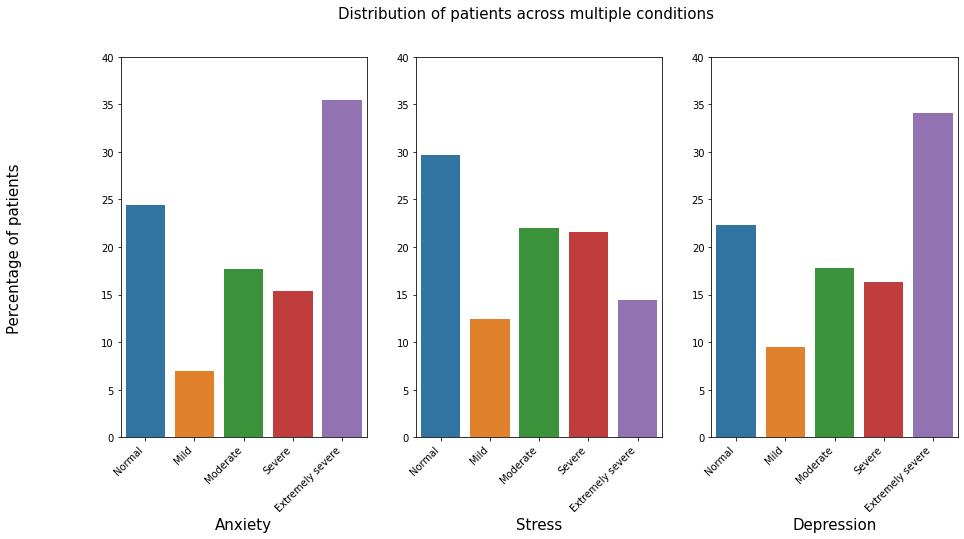
\includegraphics[scale = 0.5]{Media/Pictures/Distribution of patients across multiple conditions.png} 
\label{figure:distribution}
\end{figure}

 Se evidencia que para las condiciones de ansiedad y depresión, el mayor numero de personas se encuentra dentro del diagnostico extremadamente severo, seguido del diagnostico normal siendo el de menor preponderancia los de síntomas leves. Por otro lado la condición de estrés presenta el mayor numero de personas en el diagnostico normal, seguido por moderado y severo en forma semejante y los de menor preponderancia son leve y extremadamente severo respectivamente. Es interesante que aun cuando la condición de estrés tiene una alta correlación en su puntaje con las otras dos, las distribuciones difieren en cuanto a su diagnostico, esto se explicaría por el hecho de que los umbrales mínimos para cada condición son diferentes y esto afecta directamente la distribución de los diagnósticos. 
 \medbreak
 
Así mismo a partir del diagnostico de los pacientes, se puede calcular el perfil medio de cada diagnostico para cada condición como se evidencia en los cuadros  \ref{table:anxiety_profile}, \ref{table:depression_profile} y \ref{table:stress_profile}:
 
 


\begin{table}[ht]
\centering
\caption{Perfil medio dentro de cada diagnostico para ansiedad}
\resizebox{\textwidth}{12mm}{\begin{tabular}{lrrrrrrrrrrrrrrrrrrr}
\toprule
               diagnosis &  education &  urban &  gender &  religion &  orientation &  race &  married &  TIPI1 &  TIPI2 &  TIPI3 &  TIPI4 &  TIPI5 &  TIPI6 &  TIPI7 &  TIPI8 &  TIPI9 &  TIPI10 &   age &  familysize \\
\midrule
Normal anxiety & 3 & 3 & 2 & 10 & 1 & 10 & 1 & 4.17 & 3.80 & 5.15 & 3.81 & 5.41 & 4.42 & 5.27 & 3.67 & 4.74 & 3.42 & 26.94 & 3.48 \\
Mild anxiety & 3 & 3 & 2 & 10 & 1 & 10 & 1 & 4.01 & 4.01 & 4.89 & 4.71 & 5.17 & 4.65 & 5.28 & 4.07 & 4.10 & 3.63 & 24.09 & 3.52 \\
Moderate anxiety & 3 & 3 & 2 & 10 & 1 & 10 & 1 & 3.80 & 4.17 & 4.78 & 5.11 & 5.00 & 4.84 & 5.25 & 4.24 & 3.77 & 3.76 & 23.45 & 3.54 \\
Severe anxiety & 2 & 3 & 2 & 10 & 1 & 10 & 1 & 3.68 & 4.24 & 4.63 & 5.53 & 4.86 & 4.92 & 5.29 & 4.40 & 3.41 & 3.81 & 22.36 & 3.48 \\
Extremely severe anxiety & 2 & 3 & 2 & 10 & 1 & 10 & 1 & 3.52 & 4.49 & 4.47 & 6.08 & 4.56 & 5.16 & 5.28 & 4.71 & 2.86 & 3.92 & 21.25 & 3.50 \\
\bottomrule
\end{tabular}}
\label{table:anxiety_profile}
\end{table}%


\begin{table}[ht]
\centering
\caption{Perfil medio dentro de cada diagnostico para depresión}
\resizebox{\textwidth}{12mm}{\begin{tabular}{lrrrrrrrrrrrrrrrrrrr}
\toprule
                  diagnosis &  education &  urban &  gender &  religion &  orientation &  race &  married &  TIPI1 &  TIPI2 &  TIPI3 &  TIPI4 &  TIPI5 &  TIPI6 &  TIPI7 &  TIPI8 &  TIPI9 &  TIPI10 &   age &  familysize \\
\midrule
Normal depression & 3 & 3 & 2 & 10 & 1 & 10 & 1 & 4.45 & 3.75 & 5.34 & 3.92 & 5.49 & 4.24 & 5.41 & 3.54 & 4.91 & 3.38 & 25.38 & 3.63 \\
Mild depression & 3 & 3 & 2 & 10 & 1 & 10 & 1 & 4.13 & 4.07 & 4.99 & 4.84 & 5.20 & 4.60 & 5.35 & 4.04 & 4.16 & 3.63 & 24.16 & 3.61 \\
Moderate depression & 3 & 3 & 2 & 10 & 1 & 10 & 1 & 3.91 & 4.16 & 4.79 & 5.24 & 5.02 & 4.80 & 5.31 & 4.23 & 3.75 & 3.73 & 23.37 & 3.55 \\
Severe depression & 2 & 3 & 2 & 10 & 1 & 10 & 1 & 3.69 & 4.32 & 4.62 & 5.50 & 4.85 & 4.92 & 5.28 & 4.48 & 3.39 & 3.79 & 22.65 & 3.45 \\
Extremely severe depression & 2 & 3 & 2 & 10 & 1 & 10 & 1 & 3.24 & 4.47 & 4.32 & 5.90 & 4.50 & 5.31 & 5.14 & 4.76 & 2.76 & 3.95 & 22.27 & 3.38 \\
\bottomrule
\end{tabular}}
\label{table:depression_profile}
\end{table}%


\begin{table}[ht]
\centering
\caption{Perfil medio dentro de cada diagnostico para estrés}
\resizebox{\textwidth}{12mm}{\begin{tabular}{lrrrrrrrrrrrrrrrrrrr}
\toprule
              diagnosis &  education &  urban &  gender &  religion &  orientation &  race &  married &  TIPI1 &  TIPI2 &  TIPI3 &  TIPI4 &  TIPI5 &  TIPI6 &  TIPI7 &  TIPI8 &  TIPI9 &  TIPI10 &   age &  familysize \\
\midrule
Normal stress & 3 & 3 & 2 & 10 & 1 & 10 & 1 & 4.15 & 3.65 & 5.10 & 3.79 & 5.36 & 4.51 & 5.32 & 3.76 & 4.84 & 3.51 & 25.47 & 3.61 \\
Mild stress & 3 & 3 & 2 & 10 & 1 & 10 & 1 & 3.86 & 4.02 & 4.78 & 4.97 & 5.06 & 4.81 & 5.30 & 4.21 & 3.91 & 3.74 & 23.66 & 3.48 \\
Moderate stress & 2 & 3 & 2 & 10 & 1 & 10 & 1 & 3.72 & 4.26 & 4.67 & 5.50 & 4.90 & 4.92 & 5.28 & 4.38 & 3.45 & 3.75 & 22.80 & 3.46 \\
Severe stress & 2 & 3 & 2 & 10 & 1 & 10 & 1 & 3.58 & 4.54 & 4.55 & 6.01 & 4.69 & 5.02 & 5.24 & 4.57 & 2.91 & 3.84 & 22.16 & 3.44 \\
Extremely severe stress & 2 & 3 & 2 & 10 & 1 & 10 & 1 & 3.39 & 4.84 & 4.37 & 6.42 & 4.37 & 5.23 & 5.20 & 4.82 & 2.38 & 3.96 & 21.69 & 3.43 \\
\bottomrule
\end{tabular}}
\label{table:stress_profile}
\end{table}%

Se aprecia que algunas de estas variables cambian de valor proporcionalmente de manera a análoga en todos las condiciones: el nivel educativo tiende a ser menor para diagnósticos severos, así mismo la edad tiende a disminuir con la severidad. En cuanto al TIPI, los enunciados 1, 3, 5, y 9 tienden a disminuir, lo cual tiene sentido pues están asociados a características positivas de la personalidad como entusiasmo, disciplina, apertura a nuevas experiencias y calma. Por otro lado los enunciados 2, 4, 6 y 8 tienden a aumentar con el diagnostico; estos enunciados están a su vez asociados con características negativas de la personalidad como conflictividad, irritabilidad, reserva y desorden. 


